\documentclass[week3]{csse1001}

\title{CSSE1001 Week 3 Practicals}
 
\begin{document}

\begin{frame} 
\maketitle
\end{frame}

\section{Assignment 1 is out!}

\begin{topic}{Assignment brief}
Basic cryptography - encrypt and decrypt text using a caesar shift
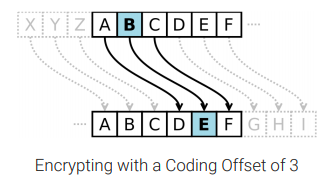
\includegraphics[scale=1]{encryption}
\end{topic}

\section{Assignment 1 demo}

\begin{topic}{Getting started}
Navigate to Blackboard $\to$ Assessment $\to$ Assignment 1\\
\vspace{1cm}
Download the following files:
\begin{itemize}
\item \code{a1.py} - the main assignment file - \textbf{write all your code in this file}
\item \code{a1\_support.py} - contains some supporting functions - download this and put it in the same directory (folder) as \code{a1.py}
\item \code{words.txt} - a list of all English words (used by the support code, so also put this in the same directory as the other two files)
\end{itemize}

\end{topic}

\begin{topic}{Writing your assignment}
You \textit{must} write the following functions as a part of your code:\\

\begin{itemize}
\item \code{encrypt(text, offset)} - Encrypts \code{text} by replacing each letter with the letter some fixed number of positions (the \code{offset}) down the alphabet. Returns the encrypted text.
\item \code{decrypt(text, offset)} - Decrypts \code{text} that was encrypted by the function above. Returns the decrypted text.
\item \code{find\_encryption\_offsets(encrypted\_text)} - Returns a tuple containing all possible offsets that could have been used if to encrypt some English text into \code{encrypted\_text}.
\item \code{main()} - Handles interaction with the user
\end{itemize}

\begin{subtopic}{2-}
See the assignment sheet for more details and examples
\end{subtopic}

\end{topic}

\begin{topic}{Extension}
There are two more challenging extension tasks for this assignment (worth 1 mark in total)\\

\begin{itemize}
\item When 0 is entered as a shift offset, display the encrypted/decrypted text for \textit{all} offsets (1-25)
\item Accept all characters (not just English letters and spaces) - i.e. characters with ASCII codes from 32 to 126
\end{itemize}

\end{topic}

\begin{topic}{Documentation}
All the functions you write for the assignment (except for \code{main}) must have a \textbf{docstring} outlining what the function does, what parameters it takes, and what it returns

\begin{subtopic}{2-}
See the \href{http://csse1001.uqcloud.net/notes/commenting}{course notes on commenting} for information on how your docstrings should be written
\end{subtopic}

\begin{subtopic}{3-}
It is also expected that any complicated parts of code are explained using \textbf{inline comments}
\end{subtopic}

\begin{subtopic}{4-}
Make sure you do not overuse comments - for example the following comment is considered extraneous and will lose marks:\\
\code{x = 1   \# x is assigned 1}
\end{subtopic}

\end{topic}

\begin{topic}{Marking criteria}
This assignment is worth 5\% of your final grade - there are 10 marks in total

\begin{subtopic}{2-}
\textbf{5 of the 10} marks are allocated to \textbf{functionality} (1 of these marks is for the extension)
\end{subtopic}

\begin{subtopic}{3-}
\textbf{2 of the 10} marks are allocated to \textbf{documentation} (i.e. docstrings and commenting)
\end{subtopic}

\begin{subtopic}{4-}
\textbf{3 of the 10} marks are allocated to \textbf{coding style} (i.e. good variable naming, readability, and appropriate logic)
\end{subtopic}

\end{topic}

\begin{topic}{Marking}
The functionality component of this assignment will me \textit{automatically marked}

\begin{subtopic}{2-}
Each of the major functions (\code{encrypt}, \code{decrypt}, \code{find\_encryption\_offsets} and \code{main}) will be tested individually
\end{subtopic}

\begin{subtopic}{3-}
Because of this, ensure the function definitions (i.e. function names and parameters) are the same as the examples on the assignment spec
\end{subtopic}

\begin{subtopic}{4-}
Also ensure the output of your code is \textit{identical} to the examples on the assignment spec
\end{subtopic}

\begin{subtopic}{5-}
It is likely that you will be given a sample test suite before your assignment is due which will be similar but \textit{not as comprehensive} as the tests we will use to mark your assignment
\end{subtopic}

\end{topic}

\begin{topic}{How to start?}
Re-read the assignment sheet so you fully-understand what we are expecting

\begin{subtopic}{2-}
Implement the \code{encrypt}, \code{decrypt}, and \code{find\_encryption\_offsets} functions first (you'll likely want to do them in that order)\\
These functions shouldn't use the \code{input} or \code{print} functions - they should only take the expected arguments and return the expected output
\end{subtopic}

\begin{subtopic}{3-}
Once you have tested these and know they are working (have a look at the examples on the assignment sheet), you can implement \code{main} (which will handle the user input and printing)
\end{subtopic}

\begin{subtopic}{4-}
Leave the extension task until the end as it's worth few marks
\end{subtopic}

\begin{subtopic}{5-}
Document your code as you go
\end{subtopic}

\end{topic}

\begin{topic}{Academic misconduct}
This is your assignment and must be 100\% your work

\begin{subtopic}{2-}
Do not share assignment code with other students
\end{subtopic}

\begin{subtopic}{3-}
Do not look at other people's code
\end{subtopic}

\begin{subtopic}{4-}
Do not discuss exact solutions to the assignment with others
\end{subtopic}

\begin{subtopic}{5-}
Do not copy large blocks of code from the internet
\end{subtopic}

\end{topic}

\end{document} 
